\section{Graph Isomorphism}

\frame{
{Part 1: Graph Isomorphism}

\tableofcontents[currentsection,hideallsubsections, firstsection=1, sections={1-4}]
}

\begin{frame}{Directed Graphs and Simple Graphs}
  \begin{columns}[T]
    \column{0.5\textwidth}
    \begin{center}
      Directed Graph:\\

      \begin{tikzpicture}[scale=.8,auto,swap]
        \tikzset{edge/.style = {->,>=latex'}}
        \node[vertex] (a) at (0,0) {a};
        \node[vertex] (b) at (2,3) {b};
        \node[vertex] (c) at (4,2) {c};
        \node[vertex] (d) at (4,0) {d};
        \draw[edge] (a) to (b);
        \draw[edge] (a) to (c);
        \draw[edge] (c) to (b);
        \draw[edge] (d) to (c);
        \draw[edge] (d) to[bend left] (a);
        \draw[edge] (a) to[bend left] (d);
        \draw[edge] (a) to[loop left] (a);
      \end{tikzpicture}
    \end{center}
    \column{0.5\textwidth}
    \begin{center}
      Simple Graph:\\

      \begin{tikzpicture}[scale=.8,auto,swap]
        %\tikzset{edge/.style = {->,>=latex'}}
        \node[vertex] (a) at (0,0) {a};
        \node[vertex] (b) at (2,3) {b};
        \node[vertex] (c) at (4,2) {c};
        \node[vertex] (d) at (4,0) {d};
        \draw[edge] (a) to (b);
        \draw[edge] (a) to (c);
        \draw[edge] (c) to (b);
        \draw[edge] (d) to (c);
        \draw[edge] (d) to (a);
      \end{tikzpicture}

      \vspace{2em}
    \end{center}
    \begin{itemize}
    \item No double edges allowed;
    \item No self-loop allowed;
    \end{itemize}
  \end{columns}
\end{frame}

\begin{frame}{Simple Graphs}{Some definitions}
  A Simple Graph \structure{$G$} consists of:
  \begin{itemize}
  \item A \emph{non-empty} set \structure{$V$} of vertices;
  \item A set \structure{$E$} of edges so that:
    \begin{itemize}
    \item Each edge has \structure{two endpoints} in $V$:
      \hfill (\alert{not an {\bf start} and an {\bf end}})

      \bigskip
    \item The order of the vertices in an edge does not matter:
      \hfill $e_1 = \{v_1,v_2\} = \{v_2, v_1\}$

      \bigskip
    \item Two vertices with an edge between them are
      \structure{adjacent}

      \bigskip
    \item An edge that connects two vertices is \structure{incident}
      to them.
      \hfill Ex: $e_1$ is \structure{incident} to $v_1$ and $v_2$
    \end{itemize}
  \end{itemize}
\end{frame}

\begin{frame}{Vertice Degrees}

    The \structure{degree} of a vertex is the \structure{number of
      incident edges}.

    \begin{center}
      \begin{tikzpicture}[scale=.8,auto,swap]
        %\tikzset{edge/.style = {->,>=latex'}}
        \node[vertex] (a) at (0,0) {a};
        \node[vertex] (b) at (2,3) {b};
        \node[vertex] (c) at (4,2) {c};
        \node[vertex] (d) at (4,0) {d};
        \draw[edge] (a) to (b);
        \draw[edge] (a) to (c);
        \draw[edge] (c) to (b);
        \draw[edge] (d) to (c);
        \draw[edge] (d) to (a);
      \end{tikzpicture}

      deg(a) = 3 \hspace{1cm} deg(d) = 2
    \end{center}

    \hfill

    \alert{Quiz:} Can you build a graph with following vertice degrees?
    \begin{itemize}
    \item 3, 2, 2, 1 (four vertices)
    \item 3, 2, 2, 2 (four vertices)
    \end{itemize}
\end{frame}

\begin{frame}{Verdice Degrees}{The Handshaking Lemma}

  {\bf Lemma:} The sum of vertice degrees in a graph is 2x the number of edges.
  \begin{equation}
    2|E| = \sum_{v\in V} \text{deg}(v)
  \end{equation}

  \begin{proof}
    \begin{itemize}
      \item Every edge in a graph connects two vertices;
      \item If we begin with a graph with 0 edges, for every edge $(v_i,v_j)$ that we add to the graph, we add 2 vertice degrees (one for $v_i$, one for $v_j$).
      \item So the total of vertices is 2 times the total of edges.
    \end{itemize}
  \end{proof}\bigskip

  Because of the lemma, it is impossible to make a graph with vertice degrees 3, 2, 2, 2.
\end{frame}

\subsection{Isomorphism}

\begin{frame}{Review: Isomorphism in graphs}{Remember: an isomorphism is an edge preserving bijection}
    \begin{columns}
      \column{0.5\textwidth}
      \begin{tikzpicture}[scale=1.5,auto,swap]
        %\tikzset{edge/.style = {->,>=latex'}}
        \node[vertex] (257) at (0,2) {257};
        \node[vertex] (122) at (1,2) {122};
        \node[vertex] (145) at (2,2) {145};
        \node[vertex] (306) at (0,0) {306};
        \node[vertex] (67) at (2,0) {67};
        \node[vertex] (99) at (1,-1) {99};
        \draw[edge] (257) to (122);
        \draw[edge] (257) to (99);
        \draw[edge] (122) to (99);
        \draw[edge] (306) to (99);
        \draw[edge] (67) to (99);
        \draw[edge] (306) to (67);
        \draw[edge] (306) to (145);
        \draw[edge] (145) to (99);
      \end{tikzpicture}

      \column{0.5\textwidth}
      \begin{tikzpicture}[scale=1.5,auto,swap]
        %\tikzset{edge/.style = {->,>=latex'}}
        \node[vertex] (257) at (0,2) {257};
        \node[vertex] (122) at (2,2) {122};
        \node[vertex] (145) at (2,-1) {145};
        \node[vertex] (306) at (1,-1) {306};
        \node[vertex] (67) at (0,-1) {67};
        \node[vertex] (99) at (1,1) {99};
        \draw[edge] (257) to (122);
        \draw[edge] (257) to (99);
        \draw[edge] (122) to (99);
        \draw[edge] (306) to (99);
        \draw[edge] (67) to (99);
        \draw[edge] (306) to (67);
        \draw[edge] (306) to (145);
        \draw[edge] (145) to (99);
      \end{tikzpicture}

    \end{columns}\bigskip

    The left and the right are \structure{the same graph}, but with different positions for the vertices.
\end{frame}

\begin{frame}{Review: Isomorphism in graphs}{Remember: Isomorphism is an edge preserving vertex bijection}
    \begin{columns}
      \column{0.5\textwidth}
      \begin{tikzpicture}[scale=1.5,auto,swap]
        %\tikzset{edge/.style = {->,>=latex'}}
        \node[vertex] (257) at (0,2) {257};
        \node[vertex] (122) at (1,2) {122};
        \node[vertex] (145) at (2,2) {145};
        \node[vertex] (306) at (0,0) {306};
        \node[vertex] (67) at (2,0) {67};
        \node[vertex] (99) at (1,-1) {99};
        \draw[edge] (257) to (122);
        \draw[edge] (257) to (99);
        \draw[edge] (122) to (99);
        \draw[edge] (306) to (99);
        \draw[edge] (67) to (99);
        \draw[edge] (306) to (67);
        \draw[edge] (306) to (145);
        \draw[edge] (145) to (99);
      \end{tikzpicture}

      \column{0.5\textwidth}
      \begin{tikzpicture}[scale=1.5,auto,swap]
        %\tikzset{edge/.style = {->,>=latex'}}
        \node[vertex] (257) at (0,2) {Aki};
        \node[vertex] (122) at (1,2) {Bob};
        \node[vertex] (145) at (2,2) {Gus};
        \node[vertex] (306) at (0,0) {Lyn};
        \node[vertex] (67) at (2,0) {Taro};
        \node[vertex] (99) at (1,-1) {Emi};
        \draw[edge] (257) to (122);
        \draw[edge] (257) to (99);
        \draw[edge] (122) to (99);
        \draw[edge] (306) to (99);
        \draw[edge] (67) to (99);
        \draw[edge] (306) to (67);
        \draw[edge] (306) to (145);
        \draw[edge] (145) to (99);
      \end{tikzpicture}

    \end{columns}\bigskip

    The left and the right are \structure{the same graph}, but with different {\bf labels} for the vertices.
\end{frame}

\begin{frame}{Isomorphism}

    \begin{itemize}
    \item Graph Isomorphism is determined solely by the edges between vertices;\bigskip

    \item Two graphs with the same edge connections are \structure{isomorphic};\bigskip

    \item Formally, wwo graphs are isomorphic if there is an \structure{Edge Preserving Matching Relation} between their vertices;\bigskip
    \end{itemize}
\end{frame}

\begin{frame}{Isomorphism}{Are these graphs Isomorphic?}

    \begin{columns}
      \column{0.5\textwidth}
      \begin{tikzpicture}[scale=1.5,auto,swap]
        %\tikzset{edge/.style = {->,>=latex'}}
        \node[vertex] (a) at (0,0) {Cow};
        \node[vertex] (b) at (2,0) {Cat};
        \node[vertex] (c) at (0,2) {Dog};
        \node[vertex] (d) at (2,2) {Pig};
        \draw[edge] (a) to (b);
        \draw[edge] (b) to (d);
        \draw[edge] (d) to (c);
        \draw[edge] (c) to (a);
        \draw[edge] (c) to (b);
      \end{tikzpicture}
      \column{0.5\textwidth}
      \begin{tikzpicture}[scale=1.5,auto,swap]
        %\tikzset{edge/.style = {->,>=latex'}}
        \node[vertex] (a) at (1,2) {Hay};
        \node[vertex] (b) at (2,0) {Tuna};
        \node[vertex] (c) at (0,0) {Beef};
        \node[vertex] (d) at (1,1) {Corn};
        \draw[edge] (a) to (b);
        \draw[edge] (b) to (d);
        \draw[edge] (d) to (c);
        \draw[edge] (c) to (a);
        \draw[edge] (c) to (b);
      \end{tikzpicture}
    \end{columns}\bigskip

    Edge Preserving Bijection:\\
    f(dog) = Beef; \hspace{2cm} f(cow) = Hay\\
    f(cat) = Tuna; \hspace{2cm} f(pig) = Corn
\end{frame}

\begin{frame}{Isomorphism}{Are THESE graphics Isomorphic? (2)}

  \begin{center}
    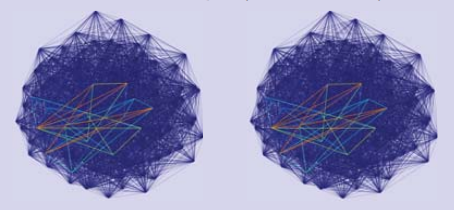
\includegraphics[width=0.8\textwidth]{../img/isomorphism}
    \pagenote{Isomorphism image from MIT OCW materials}
  \end{center}
\end{frame}

\begin{frame}{Graph Isomorphism}{Edge Preserving Bijection}

    $G_1$ \structure{isomorphic} to $G_2$ means that $\exists$
    Edge Preserving Vertex Matching:
    \begin{equation*}
      \exists f:V_1 \rightarrow V_2,
      (u,v) \in E_1 \iff (f(u),f(v)) \in E_2
    \end{equation*}\bigskip

    It is easy to quickly identify {\bf \alert{non-isomorphic}} graphs:
    \begin{itemize}
    \item Not the same number of vertices;
    \item Not the same number of edges;
    \item Not the same degree distribution;
    \item Differences in Paths, Distances, etc...
    \end{itemize}
\end{frame}

\begin{frame}{How to find Graph Isomorphism?}
    \begin{itemize}
      \item Finding the bijection is very hard:
      \begin{itemize}
        \item Total Number of possible bijections: permutation on $|V|$
        % TODO: add an example here about how to find bijections by enumerating the permutations
      \end{itemize}\bigskip

    \item If the graph is "small", can check the permutations by hand;\bigskip

    \item If the graph is "large", create random matchings $f: V_1 \rightarrow V_2$, and check:
      \begin{itemize}
        \item Quickly prune matchings that are {\bf not} isomorphic:
        \item Vertices in the bijection must have the same degree. (ex: a vertice with edge 4 must match to another vertice with edge 4)
        \item \emph{Adjacent vertices} must match degree as well. (ex: A vertice with degree 3, and neighbors with degree 4, 2, 1)
      \end{itemize}
    \end{itemize}
\end{frame}

\begin{frame}{How to find Graph Isomorphism?}

  Finding an isomorphism for two graphs is a very expensive, and important, problem. In theory, there is no algorithm that is better than just checking every possible bijection.

  \begin{center}
    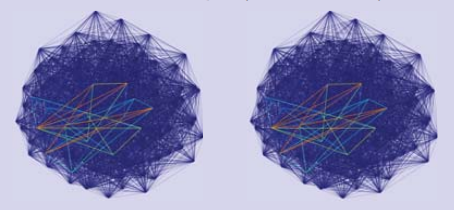
\includegraphics[width=0.8\textwidth]{../img/isomorphism}
    \pagenote{Isomorphism image from MIT OCW materials}
  \end{center}
\end{frame}
